\documentclass{article}

\usepackage{amsmath}
\usepackage{amscd}
\usepackage[tableposition=top]{caption}
\usepackage{ifthen}
\usepackage[utf8]{inputenc}
\usepackage{longtable,pdflscape} 
\usepackage{mathptmx}
\usepackage{hyperref}
\usepackage{Sweave}
\usepackage{tikz}
\usepackage{pgf}
\usepackage{a4wide}


% \VignetteIndexEntry{IPMpack: An R Package for demographic modeling}
% \VignetteDepends{Matrix, MASS, nlme, mvtnorm, methods}
% \VignetteKeyword{kwd1}
% \VignetteKeyword{kwd2}

%\SweaveOpts{prefix.string=Guide/} 
 

\title{IPMpack: an R package for demographic modeling with Integral Projection
Models (v.1.5)}
\author{Jessica Metcalf, Sean M. McMahon, Rob Salguero-Gomez, Eelke Jongejans}
\maketitle


%\section*{IPMpack: an R package for demographic modeling}
%\makeabstract
The goal of IPMpack is to provide a suite of demographic tools based
on Integral Projection Models (IPMs) to support biologists interested in
making projections for populations where demography is strongly linked to a changing continuous variable, such as size. The package includes functions that can take data, such as size or age, as well as environmental covariates, and build models of growth, survival and fecundity. Functions are defined that then take these
statistical models and construct IPMs. IPMpack has tools that compare different
functional forms for the underlying statistical models, plotting them and
returning model scores, as well as tools for diagnostic tests of the IPM models
themselves. There are also methods to build population models for varying environments, use Bayesian methods to sample population parameters,  estimate longevity and passage time, sensitivity and elasticity (of either parameters or matrix elements), and much more.

This vignette is intended to introduce the concepts of IPMs as well as the
implementation of IPMpack to biologists with a wide range of quantitative skills.  This vignette is for IPMpack version $1.5$, and so we encourage users to contact the IPMpack team at \href{IPMpack@gmail.com}{IPMpack@gmail.com} with any feedback or mistakes they find.  We also host a blog at R-forge (http://ipmpack.r-forge.r-project.org/) that contains news of updates, new features, and announcements of papers and meetings relevant to IPMs.
 
\newpage

\section{Introduction to Integral Projection Models}
An Integral Projection Model (IPM) is a demographic tool that can estimate the
dynamics of populations where individuals' fates depend on state variables that
are continuous (e.g., weight, diameter at breast height, height, limb length,
rosette diameter) or quasi-continuous (e.g., number of leaves, age, number of
reproductive structures) and may be a mixture of discrete and continuous
variables. IPMs track the distribution of individuals $n$ across these state
variables between census times (e.g., year $t$ and year $t+1$) by projecting from models that define the underlying vital rates (e.g., survival, growth, and reproduction) as a function of the (quasi-)continuous state variables. For detailed introductions to IPMs see Easterling et al. ($2000$), and Ellner \& Rees ($2006$, $2007$).

Briefly, an IPM is defined by a kernel $K$ that represents probabilities of growth between discrete or continuous stages, survival across these stages, and the production of offspring and offspring recruitment.  For example, in the simplest case, where the population is structured by a continuous covariate, size, then 
\begin{equation}
n(y, t+1) = \int\limits_{L}^{U} K(y, x) n(x, t) \, dx       
\end{equation}
where $n(y, t+1)$ is the distribution across size $y$ of both established and new individuals in census time $t+1$, $n(x, t)$ the distribution across size of individuals in census time $t$, and $L$ and $U$ the lower and upper size limits modeled in the IPM, respectively. 

Multiple functional forms for both demographic processes as well as their error
structures can be  accommodated with IPMpack. The $F$ kernel (equation 4)
describes per-capita contributions of reproductive individuals to number of new
individuals at the next census. Multiple size-dependent or size-independent
vital rates can be fitted within the $F$ kernel, reflecting for example
reproductive probability, number of reproductive structures (e.g. flowers in
plants, basidia in fungi), number of propagules within reproductive structure
(e.g. seeds in inflorescences), and so on. Additionally, a range of constants
($c_1$, $c_2$, ...) can be included if there are no data for a stage. All of these will be multiplied to obtain the eventual fertility for individuals of each size. Finally, the $F$ kernel definition includes a probability density function describing the size of offspring recruiting into the population, $f_d$. 

From equation 1: 
\begin{equation}
n(y, t+1) = \int\limits_{L}^{U} K(y, x) n(x, t) dx = \int\limits_{L}^{U}
[P(y, ) + F(y, x)] n(x, t) dx ,
\end{equation}

where

\begin{equation}
 \int\limits_{L}^{U} P(y, x) n(x, t) dx = \int\limits_{L}^{U}surv(x)growth(y, x)dx ,    
\end{equation}
and
\begin{equation}
 \int\limits_{L}^{U} F(y, x) n(x, t) dx = \int\limits_{L}^{U}
c_1 c_2 c_3 ... fec1(x)fec2(x)fec3(x)...f_d(y, x)dx     
\end{equation}
After numerically solving these kernels, key ecological and evolutionary quantities such as the population rate of increase $\lambda$, the stable population size structure, the net reproductive rate $R_0$, and many others can be estimated (see Caswell $2001$ for more a comprehensive discussion). 

Essentially, the same tools are available for IPMs as for discrete projection
matrices (matrix population models), e.g., estimation of population
growth rate, sensitivities, elasticities, life table response
experiment [LTRE] analyses, passage time calculations, etc. (Caswell
$2001$, Cochran \& Ellner $1992$, and others); as well as some
additional tools based on exploring the impact of the underlying
statistical relationships. The main difference
between an IPM and a matrix model is that while in discrete projection
matrices the number of classes (i.e., number of stages in the life
cycle of the study species) must be defined {\tt a priori}, IPMs
impose the discretization of the three-dimensional surface defined by
equation 1 in the last step for the purposes of numerical integration. This produces a typically large matrix (e.g., $100$ x $100$ cells) that is more robust to biases from matrix dimensionality (Zuidema et al. $2010$, Salguero-Gomez \& Plotkin $2010$) and sample size (Ramula et al. $2009$) than classical matrix models.

The goal of IPMpack is to provide a centralized set of quantitative techniques based on IPMs to help ecologists and evolutionary biologists model populations. IPMpack can accommodate multiple vital rates from complex life cycles all grouped into two main sub-kernels: $P$ and $F$ (equation 2) \footnote{Note than in the seminal paper by Easterling et al. ($2000$) this kernel was referred to as $P$, but here we follow the terminology by Caswell ($2001$) and call it $P$ instead). The $P$ kernel (equation 3) describes {\tt growth} between demographic censuses conditional on individuals' survival ({\tt surv}).
}.

This vignette walks through the steps of a basic IPM analysis.  We first
describe the kind of data necessary to build an IPM.  If a user begins `from
scratch', they must input data in a specific format (described below).  However
it is possible to jump past this step and use IPMpack capabilities on IPMs that
were developed outside of IPMpack. That is, if a user wants quick figures, summary statistics, other analyses on an IPM matrix already built, IPMpack can readily accommodate that.   However there are some features that, because of the object-oriented coding, require some specific structures (and other features that do not).  Please refer to the manual files, and the rest of this vignette for this information. The vignette will begin with data input.  We will then walk through how to build and analyse a basic IPM model.  More complex models will be introduced later, as well as run comparative model testing and Bayesian implementations.

\section{Getting started: setting up the data for IPMpack}
For users who prefer to define IPM matrices using their own
statistical tools, there is no requirement for the data to be in any
particular format, and most of the functions in IPMpack will operate
on the matrices directly (e.g., life expectancy, sensitivity of matrix
elements, etc.).  However, to use IPMpack's full capacities, the
individual-level demographic data must be organized in a {\tt data frame} (a
class of object in R [see help file for `data.frame' in base]), where each row
represents one observation of an organism in the population at one census time
$t$ with the following potential column names:
\begin{itemize}
\item  {\tt size}: size of individuals in census time $t$  $^*$
\item  {\tt sizeNext}: size of individuals in census time $t+1$  $^*$
\item  {\tt surv}: survival of individuals from census time $t$ to  $t+1$ (contains: 0 for death or 1 for survival) $^*$
\item  {\tt fec1, ...}: as many columns as desired relating size to sexual reproduction. For example, this might be: 
  \begin{itemize}
  \item {\tt fec1}: probability of reproduction (output: 0 for no reproductive or 1 for reproductive)
  \item {\tt fec2}: number of reproductive structures (output: 1, 2, 3, $...$) when individual is reproductive, that is, when fec1 = 1
  \item {\tt fec3}: number of propagules (output: 1, 2, 3, $...$) per reproductive structure (e.g. seeds per flower in reproductive plant individual)
  \item ...
  \end{itemize}
\item  {\tt stage}: stage of individuals in census time $t$, used to
  distinguish discrete and continuous stages, etc. For rows in the  data frame where {\tt size} is not an NA, then this must be the word ``continuous''. Where {\tt size} is NA, any variety of named discrete stages  may be defined (e.g. ``seed bank''). If this column is missing, many procedures in IPMpack are designed to simply fill in this column assuming that only ``continuous'' state variables describe the life cycle of the species, i.e. there are no discrete stages. For running {\tt makeFecObj}, the column must be a factor. If not supplied, the function will generate this column assuming all individuals are "continuous".
\item  {\tt stageNext}: stage of individuals in census time $t+1$, in the
simples case, ``continuous'' or ``dead''(which is redundant with ``0''
in the {\tt surv} column. As above, this column is not essential
for many procedures in  IPMpack. For running {\tt makeFecObj}, the column must be a factor. If not supplied, the function will generate this column assuming all individuals that are alive are ``continuous".
\item  {\tt number}: number of individuals corresponding to each row in the data frame. For all rows corresponding to movement between continuous stages, this value will be $1$, but for movement between  discrete stages (e.g., from ``dormant seeds'' to ``seeds ready to  germinate'') then this number may be $>1$, potentially directly  reflecting observed individuals in the data. This information avoids having a data frame with a row for every discrete stage (e.g. seed). As above, many  procedures in IPMpack will simply assume that this value is always 1. 
\item  {\tt covariate}: value of a discrete covariate in census time  $t$, such as light environment at time $t$, age at $t$, patch at $t$, etc. 
\item  {\tt covariateNext}: value of a discrete covariate in census time $t+1$.
\item  ...any other covariates of interest, named as desired by the user are possible too (e.g., precipitation, habitat, temperature, etc).
\item {\tt offspringNext}: if the size contained in sizeNext corresponds to the
size of an offspring, this column will contain either the value ``sexual" or
``clonal" (depending on whether sexual or clonal reproduction is being
considered). If this column exists, rows that take these two values will be excluded from the growth analyses (functions {\tt makeGrowthObj} and variants thereof, see below).
\end{itemize}

The $^*$ symbol above indicates the minimum columns in the data frame required to obtain passage time and life expectancy calculations. These values form the $P$ kernel. If sufficient additional columns are available, a full life-cycle model, containing the $F$ kernel, can be produced and further analyses are possible.  Although {\tt size} and {\tt sizeNext} can be transformed, many of the utility functions assume no transformations in columns in the original data frame pertaining to fertility. Transformations can be formally called in various parts of the package and appropriate $F$ matrices built that account for these transformations. 

\section{The basics: building an IPM}

First, the user must install IPMpack from CRAN using
{\tt install.packages("IPMpack")} and then load IPMpack into an R session
({\tt library(IPMpack)}) (see help files for problems with installation or loading). 

\begin{Schunk}
\begin{Sinput}
> library("IPMpack")
\end{Sinput}
\end{Schunk}
Next, the user must input demographic data. As mentioned above, most functions of IPMpack require a data file with at minimum columns called {\tt size}, {\tt sizeNext}, {\tt surv}, where `size' is size at time t, `sizeNext' is size one census later, and `surv' is a series of 0s and 1s, indicating if the individual survived or not. In the case of `size' and `sizeNext', data can be transformed (e.g., onto a log scale), if appropriate via functions built into IPMpack. For the purpose of learning how to use IPMpack, the user can either use his/her own data (adjusted to have the appropriate headings, as aforementioned), or generate them with a function built into IPMpack:

\begin{Schunk}
\begin{Sinput}
> dff <- generateData()
\end{Sinput}
\end{Schunk}
A quick check indicates that this contains sensible (fictional) information: 
\begin{Schunk}
\begin{Sinput}
> head(dff)
\end{Sinput}
\begin{Soutput}
      size sizeNext surv covariate covariateNext       fec      stage
1 4.574771 4.833067    1         1             0 11.071777 continuous
2 2.513680       NA    0         0             0  0.000000 continuous
3 5.564809       NA    0         1             1  1.542682 continuous
4 4.194437 3.696870    1         0             0  9.889067 continuous
5 3.719495 1.658802    1         1             0  0.000000 continuous
6 2.366873 1.710754    1         1             0  0.000000 continuous
   stageNext
1 continuous
2 continuous
3 continuous
4 continuous
5 continuous
6 continuous
\end{Soutput}
\end{Schunk}

for simplicity, no discrete covariates are included in this first example. Figure~\ref{fig:zero} (p.~\pageref{fig:zero}) is produced by the following code:

\begin{Schunk}
\begin{Sinput}
> plot(dff$size, dff$sizeNext, xlab = "Size at t", ylab = "Size at t+1")
\end{Sinput}
\end{Schunk}
\begin{figure}
\begin{center}
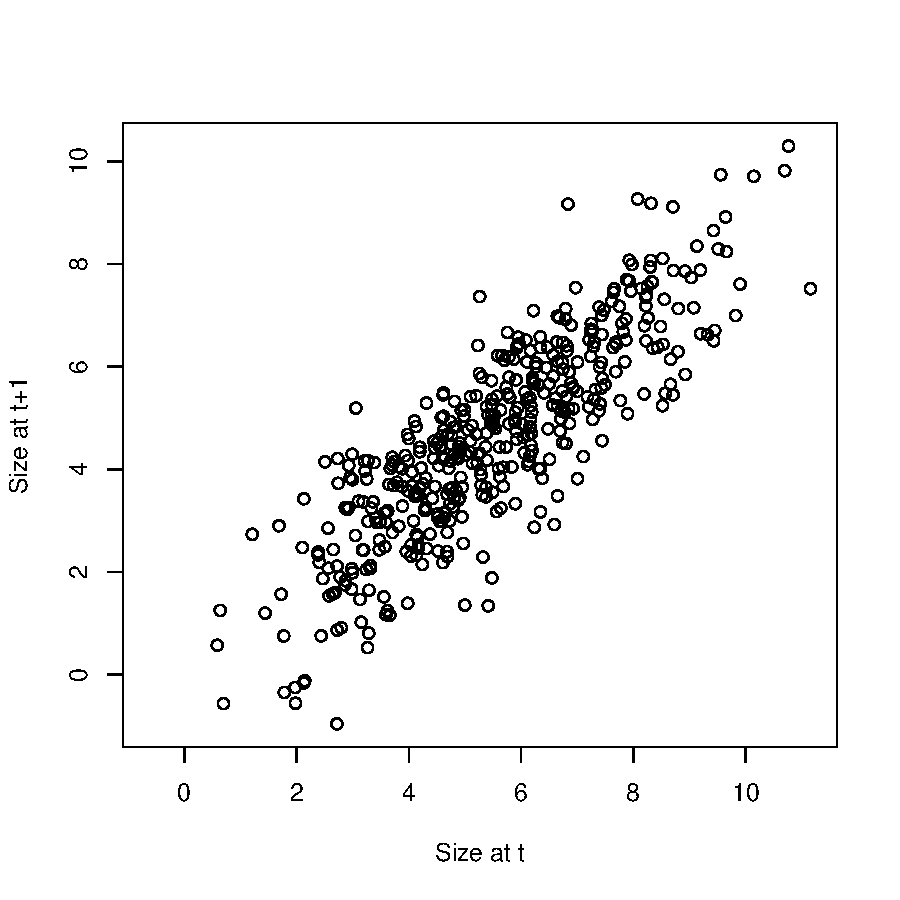
\includegraphics{IPMpack_Vignette-fig0}
\end{center}
\caption{Size at t and size at t+1}
\label{fig:zero}
\end{figure}

IPMpack is written in object-oriented code, using $S4$ objects. This means that
extra object classes are used by IPMpack, with methods assigned to those classes
that do particular things to specific objects. An example for those familiar
with $R$ is the {\tt plot} function. When applied to two vectors, it produces an x-y plot, but when applied to a fitted linear regression, it provides a series of diagnostic plots. In other words, the `plot' method is object-specific and does different things to objects of class `numeric' and objects of class `lm'.

IPMpack contains defined classes for growth, survival and fertility objects, and
associated methods that allow the user to build IPM objects. In addition, this
object-oriented structure in IPMpack uses methods from IPM objects to calculate
life expectancy, passage times, and other population estimates of interest. The
advantage of object-oriented programming is its flexibility: for example, the
same machinery can be applied to suites of underlying regression forms and the
user can take advantage of pre-existing highly generalized $R$ functions, such
as {\tt predict}. The needs of any particular dataset may require different
object and method definitions. Towards the end of this vignette we also describe how to define a new class and a new method (e.g., a new growth object for a specific life-history structure, and a new growth method applicable to plotting information from that object).

As an example, let us first define objects built as simple polynomial regressions from the generated data. The source code of {\tt generateData} will confirm that the survival data is built around a polynomial logistic regression relating size at $t$ to survival from $t$ to $t+1$, and the growth data is built around a polynomial regression relating size at $t$ to size at $t+1$. To make growth and survival objects that reflect this, the user must implement:  
\begin{Schunk}
\begin{Sinput}
> gr1 <- makeGrowthObj(dataf = dff, Formula = sizeNext~size+size2)
> sv1 <- makeSurvObj(dff, Formula = surv~size+size2)
\end{Sinput}
\end{Schunk}
In both these functions, the argument {\tt Formula} contains formulas of the type used in linear or logistic regressions in $R$, built around the possible defined range of transforms of  {\tt size} currently available ({\tt size2} which is size$^2$, {\tt size3} which is size$^3$, and {\tt logsize} which is log(size). Currently further transforms of  {\tt size} are not possible. This function can also be used to fit models that include a single discrete covariate (e.g., light environment, age, etc) as long as this exists in the {\tt dataf} in a column named {\tt covariate}. For instance, the user could model the population dynamics according to  {\tt size + covariate} or  {\tt size + logsize*covariate}, etc. For more complex analyses, other covariates (time since fire, precipitation, etc) can be fitted as long as they exist within {\tt dataf}. For the growth model, possibilities for the response variable in the {\tt Formula} are: {\tt sizeNext} meaning that the reponse variable is size at the next census time, or {\tt incr} meaning that the response variable is the size increment that has accrued between the two census times (common among tree demographic studies), and {\tt logincr} meaning that the response variable is the log of the size increment that has acrrued between the two census intervals.

Glancing at the source code will confirm that all these functions simply fit a linear regression relating size at t+1 or increment to size at t and covariates for growth, as for survival. The survival and growth objects created have a slot called `fit' that holds the regression and a slot sd that holds the variance around the regression. 
\begin{Schunk}
\begin{Sinput}
> gr1
\end{Sinput}
\begin{Soutput}
An object of class "growthObj"
Slot "fit":

Call:
lm(formula = Formula, data = dataf)

Coefficients:
(Intercept)         size        size2  
   0.337538     0.784388     0.003991  


Slot "sd":
[1] 1.054815
\end{Soutput}
\end{Schunk}
Note that before building growth or survival objects in IPMpack, careful model assessement and comparison are recommended, using all the usual regression tools available in R (plotting the fitted {\tt lm} or {\tt glm} to check for patterns of residuals, outliers etc). IPMpack also contains two functions that allow the user to check these two relationships against the data used for them in order to explore goodness of fit and effect of mesh size, shown in Figure~\ref{fig:one} (p.~\pageref{fig:one}).
\begin{Schunk}
\begin{Sinput}
> par(mfrow = c(1, 2), bty = "l", pty = "m")
> p1 <- picGrow(dff, gr1)
> p2 <- picSurv(dff, sv1, ncuts = 30)
\end{Sinput}
\end{Schunk}
\begin{figure}
\begin{center}
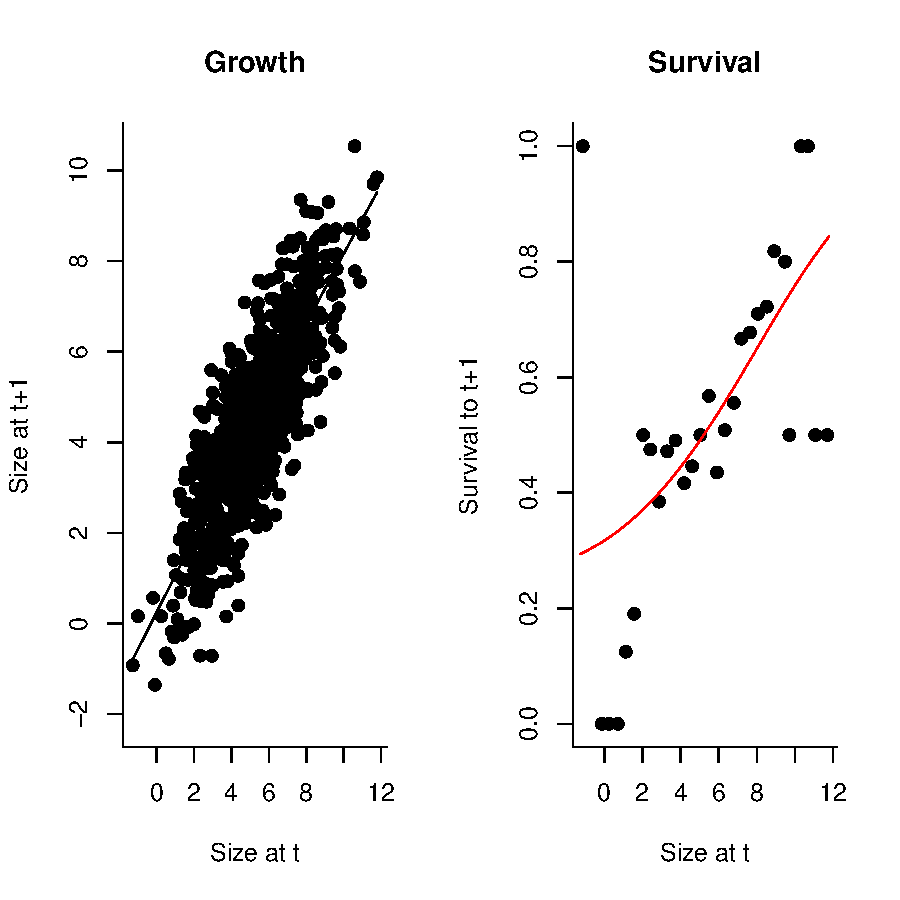
\includegraphics{IPMpack_Vignette-fig1}
\end{center}
\caption{Growth and survival objects}
\label{fig:one}
\end{figure}
To build a demographic model describing survival and growth transitions from these objects, the user can use the function {\tt createIPMPmatrix}, i.e.: 
\begin{Schunk}
\begin{Sinput}
> Pmatrix <- createIPMPmatrix(nBigMatrix = 50, 
+                             minSize = -5, maxSize = 35, 
+                             growObj = gr1, survObj = sv1, 
+                             correction = "constant")
\end{Sinput}
\end{Schunk}
where {\tt nBigMatrix} is the numbers of bins used, {\tt minSize} and
{\tt maxSize} define the limits of the IPM, $U$ and $L$ in the
equations above. Typically, these ranges should usually extend to beyond the
smallest and largest size measurement, but the user might want to exclude
outliers). The objects {\tt growObj} and {\tt survObj} define changes in size
and survival as defined above. 

\begin{figure}
\begin{center}
\begin{Schunk}
\begin{Soutput}
[1] "Range of Pmatrix is "
[1] 3.635838e-281  2.731324e-01
[1] "Please hit any key for the next plot"
\end{Soutput}
\end{Schunk}
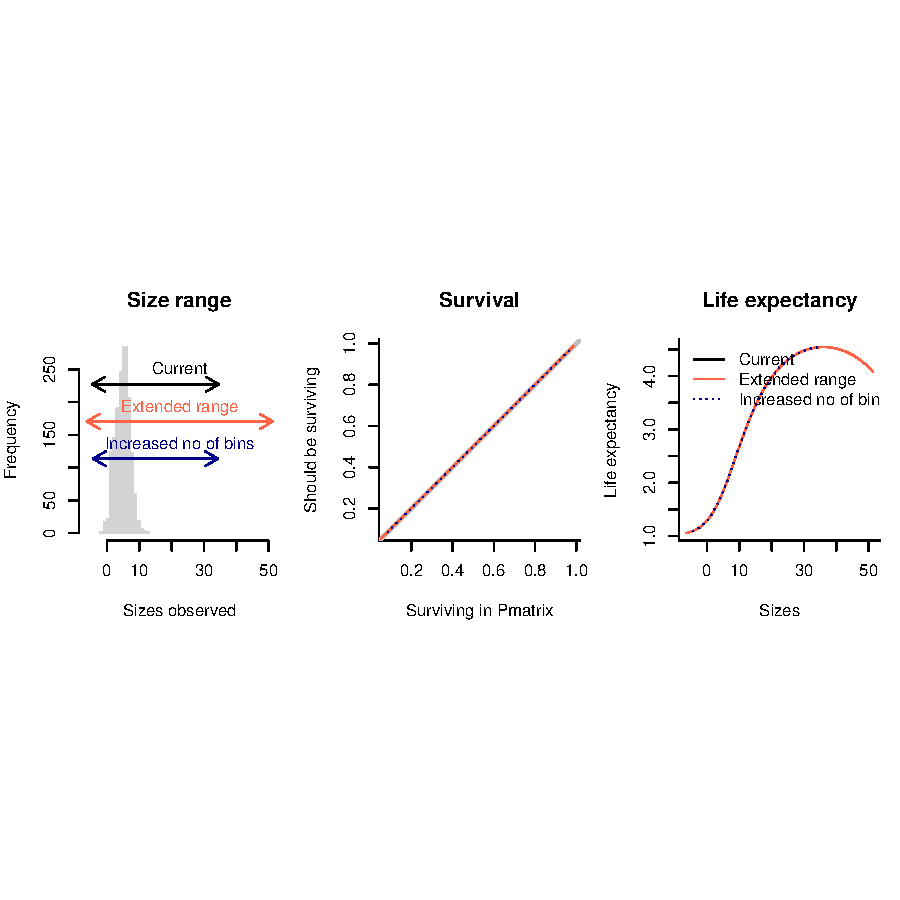
\includegraphics{IPMpack_Vignette-triDiag}
\end{center}
\caption{Diagnostic plots for the Pmatrix.}
\label{fig:triDiag}
\end{figure}

IPMpack includes a useful function {\tt diagnosticsPmatrix} that provides a
series of plots indicative of whether bin choice and size range is adequate.
Applying this function as a preliminary step before obtaining demographic and evolutionary output from IPMs can help identify basic problems in the fitting of vital rate functions or in the creation of the IPM matrices before proceeding. Several common problems can be diagnosed with the panelled figure produced by {\tt diagnosticsPmatrix} (Figure
\ref{fig:triDiag}).

The left panel on the first plot shows the range of the data (if the data is provided) and the range of the state variable fitted in the matrix (top line, black).  If these are mis-matched, the limits of the data used in building the Pmatrix can be adjusted with the {\tt minSize} and {\tt maxSize} arguments in {\tt createIPMPmatrix}.  The range for two additional Pmatrices that will be used in subsequent comparisons is also provided; one with an increased size range (red) and one with an increased number of bins (blue). 

The discretization of a continuous function can result in under- or over-estimation of the true density. Where this is occurs, the sum of the columns of the discretized matrix will not match predictions from the fitted survival model.  The middle panel 
plots these against each other for the three matrices in the first panel (current, extended range and increased bin number) using the same colours as in the first panel. Lines should fall along the (0,1) line shown in grey; if they do not, the argument {\tt correction="constant"} in {\tt createIPMPmatrix} may be of use. This ensures that the columns sum to the fitted survival by multiplying every column in the Integral Projection Model by the value that allows this. The third panel checks whether extending the size range included in the matrix and increasing the number of bins (by increasing {\tt nBigMatrix} and thereby having narrower bins) does not alter basic predictions from the IPM.

The six panels on the next plot (that may not be present in the pdf of the vignette, but should appear if you run the function) show the discretized IPM (histograms)for the current IPM (top) and one with an increased number of bins (bottom)  and the
theoretical density function (red line). These are plotted either for three chosen sizes ({\tt sizesToPlot}) or the 0.25, 0.5 and 0.75 quantiles of either the observed data (if supplied) or the range of meshpoints (if not); this size is printed in the top right hand of every plot. If the theoretical density function curve is very distant from the histograms, increasing the {\tt nBigMatrix} argument may correct this discrepancy. 

Other useful function for verifying that sufficient bins have been used include {\tt convergeLambda} and associated functions; see the help file and try them out. 

The {\tt createIPMPmatrix} function builds around methods defined so that it
will provide appropriate output whatever the survival and growth objects are
(e.g. error structure, covariates). The P matrix contains a matrix defining the
transitions, but also other useful slots, e.g., the meshpoints, covariates,
grid size. The user can access this information by writing:
\begin{Schunk}
\begin{Sinput}
> slotNames(Pmatrix)
\end{Sinput}
\begin{Soutput}
[1] ".Data"          "nDiscrete"      "nEnvClass"      "nBigMatrix"    
[5] "meshpoints"     "env.index"      "names.discrete"
\end{Soutput}
\end{Schunk}
and obtain the slots by using the $@$ symbol, e.g., 
\begin{Schunk}
\begin{Sinput}
> Pmatrix@meshpoints
\end{Sinput}
\begin{Soutput}
 [1] -4.6 -3.8 -3.0 -2.2 -1.4 -0.6  0.2  1.0  1.8  2.6  3.4  4.2  5.0  5.8  6.6
[16]  7.4  8.2  9.0  9.8 10.6 11.4 12.2 13.0 13.8 14.6 15.4 16.2 17.0 17.8 18.6
[31] 19.4 20.2 21.0 21.8 22.6 23.4 24.2 25.0 25.8 26.6 27.4 28.2 29.0 29.8 30.6
[46] 31.4 32.2 33.0 33.8 34.6
\end{Soutput}
\end{Schunk}
Finally, the user can plot the Pmatrix using {\tt persp} or {\tt
  image} (Figure~\ref{fig:two}). 
\begin{figure}
\begin{center}
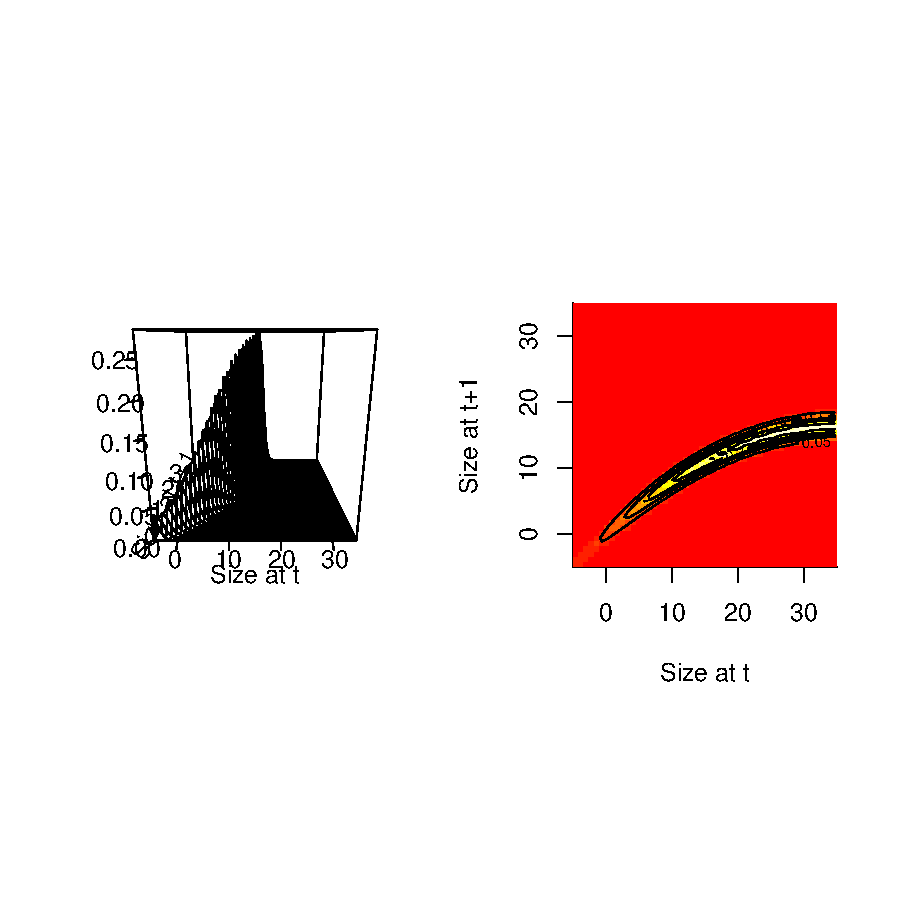
\includegraphics{IPMpack_Vignette-fig2}
\end{center}
\caption{Transition matrix encompassing survival and growth transitions only}
\label{fig:two}
\end{figure}
%Cory says: add image, makes it easier to compare to sensitivities and elasticities
Next, with this, the user can obtain the life expectancy, and passage time to a chosen size (here set at the mean) for the range of meshpoints
\begin{Schunk}
\begin{Sinput}
> LE <- meanLifeExpect(Pmatrix)
> pTime <- passageTime(mean(dff$size, na.rm = TRUE), Pmatrix)
\end{Sinput}
\end{Schunk}
and the user can also plot these against {\tt Pmatrix@meshpoints} to examine how
life expectancy and passage vary as a function of size (Figure~\ref{fig:three} p.~\pageref{fig:three}).
\begin{figure}
\begin{center}
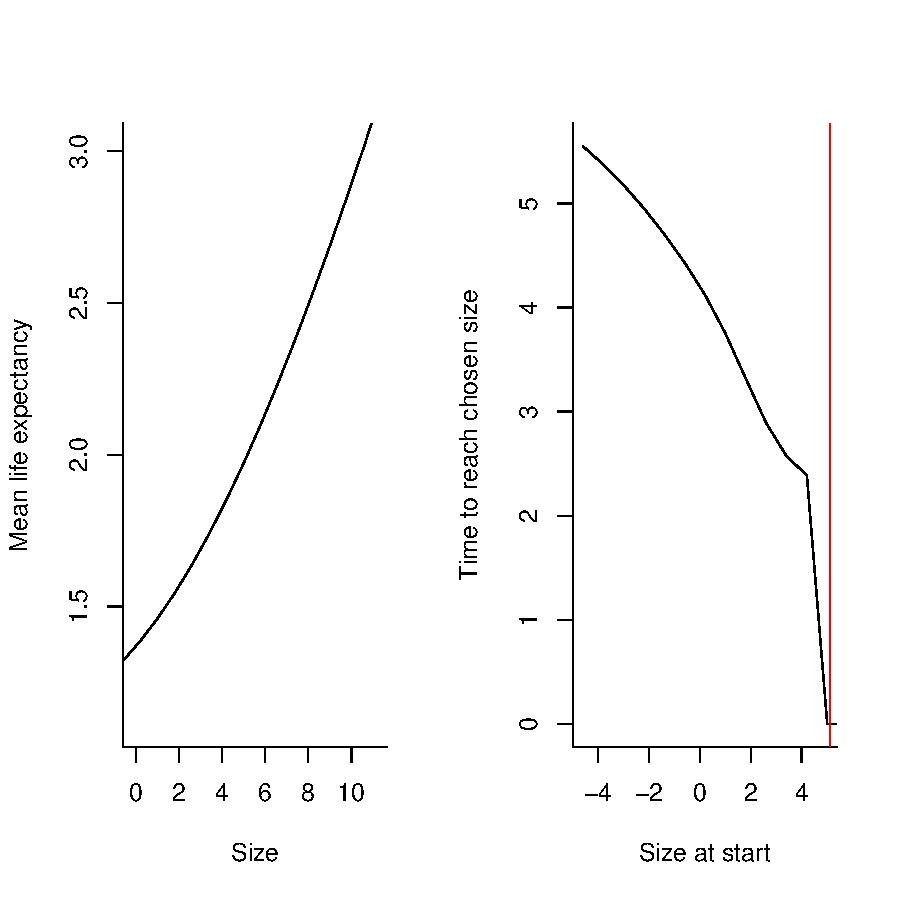
\includegraphics{IPMpack_Vignette-fig3}
\end{center}
\caption{Associated Life Expectancy and Passage Time}
\label{fig:three}
\end{figure}
The function {\tt runSimpleModel} takes as minimum arguments a data frame and a
target size (i.e., here type: {\tt runSimpleModel(dff, chosenSize = 4)}) and runs this analysis to create figures for survival, growth, life expectancy and passage time as shown so far, assuming the simplest possible models of survival and growth (basic linear and logistic regressions, no covariates except for size, etc).

If the user defines a fertility object - which, for instance, is not always easy with for example trees - IPMpack can also create a transition matrix describing movement between sizes attributable to fertility.
\begin{Schunk}
\begin{Sinput}
> fv1 <- makeFecObj(dff, Formula = fec~size, 	
+                   Family = "gaussian", 
+                   Transform = "log")
> Fmatrix <- createIPMFmatrix(nBigMatrix = 50, minSize = -5,
+                             maxSize = 35, 
+                             fecObj = fv1, 
+                             correction = "constant")
\end{Sinput}
\end{Schunk}
Note that {\tt makeFecObj} will use the relationships defined in {\tt Formula} and the family defined in {\tt Family} with transforms defined in {\tt Transform} in the order supplied. Please note that the fecundity {\tt Formula} MUST match the {\tt Transform} since IPMPack needs to combine the parameters from  {\tt Formula}  with the right  {\tt Transform}  to appropriately build the F matrixs. 

The default arguments required to run {\tt makeFecObj} to create a fecundity
object from which an F matrix with no discrete stage can be built are {\tt
offspringSplitter=data.frame(continuous=1)}, {\tt 
vitalRatesPerOffspringType=data.frame(NA)} and {\tt fecByDiscrete=data.frame(NA)}.
Additionally, note that if there are values other than ``{\tt continuous}" in the {\tt stage} column of the data-frame named {\tt dff} in the example above, then the function will assume that multiple offspring classes are required, and the result will be an IPM with nBigMatrix + the number of offspring classes deduced (which is the number of names in {\tt stage} other than ``{\tt continuous}"). This may lead to a mismatch with the size of the P matrix unless a discrete transition matrix is explicitly being included in the P matrix (see below, incorporating discrete stages).

If the data-frame contains an extra column {\tt offspringNext} that takes the
values {\tt sexual}, and that corresponds to rows where both {\tt size} and {\tt sizeNext} are different from NA, the user can define a relationship between maternal size and offspring size through the {\tt makeFecObj} argument {\tt offspringSizeExplanatoryVariables}. The default is to only fit an intercept, equivalent to simply having a mean and variance of offspring size. The function {\tt makeFecObj} also allows users to simply over-write the mean and variance of offpsring size with the values of their choice (arguments {\tt meanOffspringSize} and {\tt sdOffspringSize}).

The function {\tt makeClonalObj} operates identically to {\tt makeFecObj} except that offspring are only considered for fitting the distribution of mean and standard deviation of offspring size if the column {\tt offspringNext} takes the values {\tt clonal}. Rows where {\tt offspringNext} takes the values ``sexual" or ``clonal" are excluded from the survival and growth analyses ({\tt makeGrowthObj} and {\tt makeSurvObj}).

The user can combine the F matrix with (an identically built, i.e., same bin number, size limits and discrete classes) survival-growth transition P matrix to obtain a full Integral Projection Model, and its population growth rate $\lambda$, sensitivity, elasticity, etc. 
\begin{Schunk}
\begin{Sinput}
> IPM <- Pmatrix + Fmatrix
> Re(eigen(IPM)$value[1])
\end{Sinput}
\begin{Soutput}
[1] 3.179538
\end{Soutput}
\begin{Sinput}
> sensitivity <- sens(IPM)
> elasticity <- elas(IPM)
\end{Sinput}
\end{Schunk}
These outputs can be plotted against the meshpoints (Figure~\ref{fig:four} p.~\pageref{fig:four}).
\begin{figure}
\begin{center}
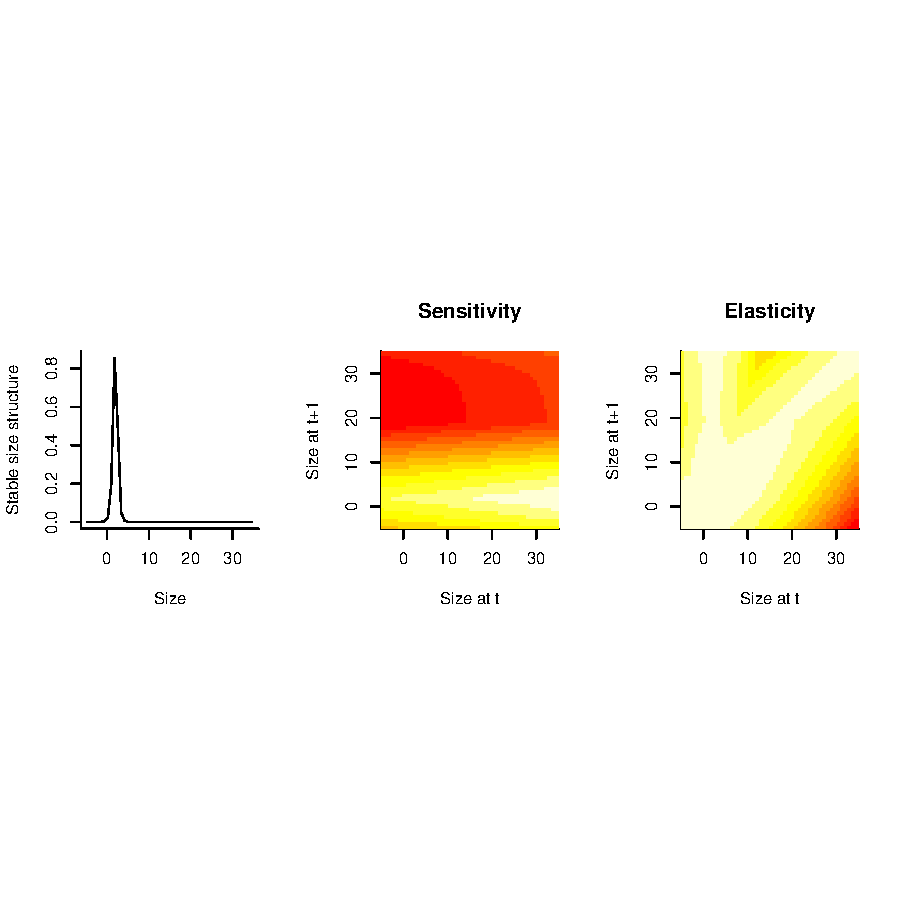
\includegraphics{IPMpack_Vignette-fig4}
\end{center}
\caption{Measures off a full IPM}
\label{fig:four}
\end{figure}
In addition to perturbation measures from mesh cells, the user can also obtain sensitivity and elasticity of particular parameters that underlie the kernels, e.g., doing:
\begin{Schunk}
\begin{Sinput}
> res <- sensParams(growObj = gr1, survObj = sv1, fecObj = fv1, 
+                   nBigMatrix = 50, minSize = -5, maxSize = 15)
> res
\end{Sinput}
\begin{Soutput}
$slam
         grow (Intercept)                 grow size                grow size2 
               0.08899972                0.19481022                0.45605382 
                sd growth          surv (Intercept)                 surv size 
               0.02587690                0.21820648                0.47138917 
               surv size2 offspring rel (Intercept)              sd offspring 
               1.08817461                0.79493601                0.09999890 
     reprod 1 (Intercept)             reprod 1 size 
               2.86194406                6.13164832 

$elam
         grow (Intercept)                 grow size                grow size2 
             0.0094384432              0.0480100553              0.0005717901 
                sd growth          surv (Intercept)                 surv size 
             0.0085758673             -0.0949064747              0.0445232287 
               surv size2 offspring rel (Intercept)              sd offspring 
            -0.0021013399              0.5153040741              0.0142892022 
     reprod 1 (Intercept)             reprod 1 size 
             0.4513885922              0.5067163359 
\end{Soutput}
\end{Schunk}
and this output can be plotted out (Figure~\ref{fig:foura} p.~\pageref{fig:foura}) using
\begin{Schunk}
\begin{Sinput}
> par(mfrow = c(2, 1), bty = "l", pty = "m")
> barplot(res$slam, main = expression("Parameter sensitivity of "*lambda), 
+ 		    las = 2, cex.names = 0.5)
> barplot(res$elam, main = expression("Parameter elasticity of "*lambda), 
+ 		    las = 2, cex.names = 0.5)
\end{Sinput}
\end{Schunk}
\begin{figure}
\begin{center}
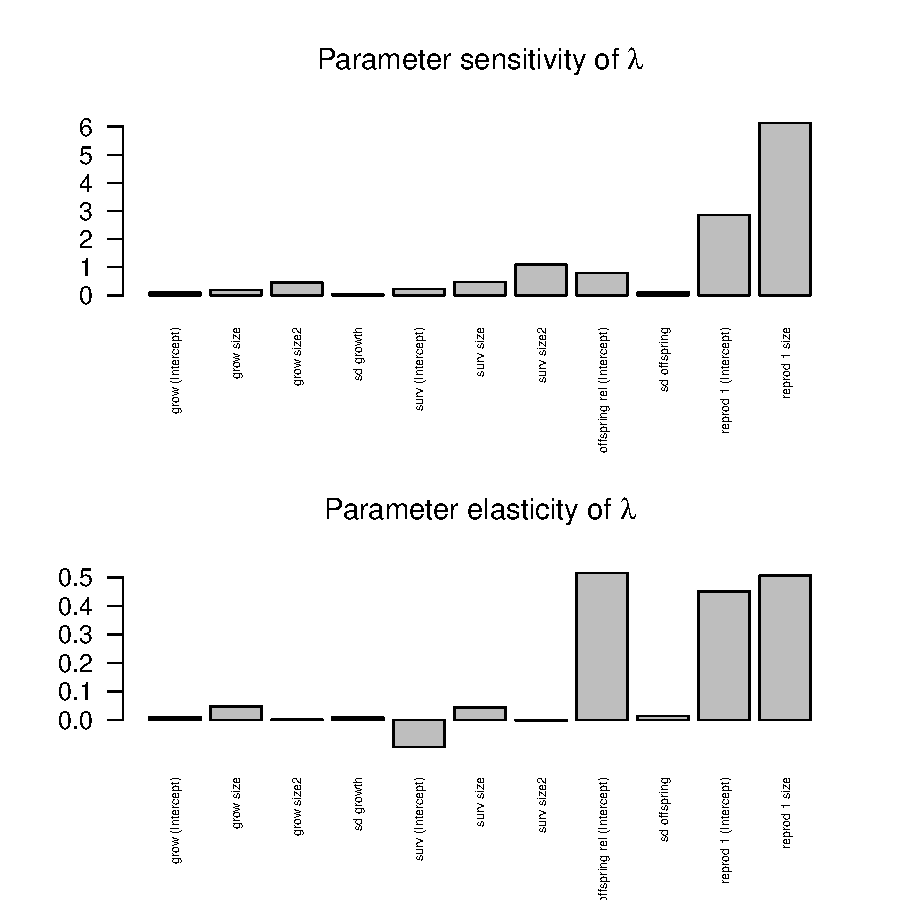
\includegraphics{IPMpack_Vignette-fig4a}
\end{center}
\caption{Sensitivity and elasticity of parameter values}
\label{fig:foura}
\end{figure}
%Similar code could be developed to explore sensitivity of other emergent %measures, e.g., mean passage time, etc. 


\section{Incorporating discrete stages}
Populations are often structured by both discrete and a continuous stages.  For
example, many plant populations may persist for many years in a seedbank as well
as having size-determined fates after they germinate. IPMpack can incorporate
this variability for complex life cycles (Ellner \& Rees $2006$). To illustrate
using discrete stages in an IPM, we generate data that includes
both discrete and continuous life-history stages:
\begin{Schunk}
\begin{Sinput}
> dff <- generateDataDiscrete()
\end{Sinput}
\end{Schunk}
A quick check indicates that these data contain several types of stage classification (and not just "continuous" as seen up till now):
\begin{Schunk}
\begin{Sinput}
> table(dff$stage)
\end{Sinput}
\begin{Soutput}
continuous    dormant   seedAge1    seedOld 
       950         50         35         32 
\end{Soutput}
\end{Schunk}
Given this data structure, the user can make a fertility object that reflects the
fact that propagules (seeds in this example) produced in one year may 
recruit directly into the continuous phase (e.g., seedling), or may end up in a
discrete stage (e.g., seed bank). The {\tt makeFecObj} (and similar functions)
has an argument called {\tt offspringSplitter} that allows the user to define
these paths:
\begin{Schunk}
\begin{Sinput}
> fv1 <- makeFecObj(dataf = dff, Transform = "log", 
+                   offspringSplitter = data.frame(continuous = 0.2, 
+                   dormant = 0, seedAge1 = 0.8, seedOld = 0), 
+                   fecByDiscrete = data.frame(dormant = 0, 
+                   seedAge1 = 0, seedOld = 0))
\end{Sinput}
\end{Schunk}
In this example, 20\% of seeds produced at $t$ end up in the continuous part of
the population structure at $t+1$ (for example, they might directly recruit as
rosettes from one year to the next) and 80\% of seeds recruit into the "one year
old seeds" stage. Although in this case no individuals are recruited at $t+1$
into the "dormant" or "old seeds" stages (since these will come from adult
plants or the seed bank), they are included because {\tt offspringSplitter} is
where IPMpack identifies all the existing discrete stages. The argument {\tt fecByDiscrete} reflects the fact that none of the discrete classes addressed in this example are likely to directly produce offspring (which may not always be the case). The resulting fecundity object can be used with {\tt createIPMFmatrix} in the usual way:
\begin{Schunk}
\begin{Sinput}
> Fmatrix <- createIPMFmatrix(fecObj = fv1, nBigMatrix = 5, 
+                             minSize = min(dff$size, na.rm = TRUE), 
+                             maxSize = max(dff$size, na.rm = TRUE), 
+                             correction = "constant")
\end{Sinput}
\end{Schunk}
The user also needs a {\tt Pmatrix} that reflects the same structure. The
continuous part of the P matrix will be the standard structure:
\begin{Schunk}
\begin{Sinput}
> gr1 <- makeGrowthObj(dataf = dff, 
+                       Formula = sizeNext~size)
> sv1 <- makeSurvObj(dff,  Formula = surv~size)
\end{Sinput}
\end{Schunk}
Movement in and out of discrete stages is defined via an add-on of a transition matrix, that is defined using: 
\begin{Schunk}
\begin{Sinput}
> discTrans <- makeDiscreteTrans(dff)
\end{Sinput}
\end{Schunk}
which captures survival and transitions between discrete stages and the
continuous stage (note that this function will not work unless the data frame
{\tt dff} contains appropriate columns {\tt stage} and {\tt stageNext}).  The
user can then construct the P matrix:
\begin{Schunk}
\begin{Sinput}
> Pmatrix <- createIPMPmatrix(nBigMatrix = 5, 	
+                             growObj = makeGrowthObj(dff), 
+                             survObj = makeSurvObj(dff), 
+                             discreteTrans = discTrans, 
+                             correction = "constant")
\end{Sinput}
\end{Schunk}
Note that both the P matrix and the F matrix in this example have a rather small number of bins just for ease of comparison, and that a higher number is almost certainly advisable. The user can examine both matrices: 
\begin{Schunk}
\begin{Sinput}
> print(Pmatrix)
\end{Sinput}
\begin{Soutput}
An object of class "IPMmatrix"
             [,1]          [,2]         [,3]          [,4]          [,5]
[1,] 2.200000e-01  0.000000e+00 0.000000e+00  1.678805e-02  6.572653e-01
[2,] 0.000000e+00  0.000000e+00 0.000000e+00  0.000000e+00  0.000000e+00
[3,] 0.000000e+00  4.439560e-01 4.323308e-01  0.000000e+00  0.000000e+00
[4,] 7.798691e-01  7.252747e-02 1.127819e-01  4.201495e-01  7.591321e-17
[5,] 1.308880e-04  4.586075e-11 9.830391e-09  2.816979e-24  5.822860e-03
[6,] 2.545958e-21  2.361411e-36 3.827338e-27  4.544024e-95  1.074565e-36
[7,] 5.739524e-51  9.901334e-78 6.656066e-57 1.763496e-213 4.770960e-118
[8,] 1.499594e-93 3.380708e-135 5.170508e-98  0.000000e+00 5.096313e-247
              [,6]          [,7]          [,8]
[1,]  6.408338e-01  3.663507e-01  6.276229e-02
[2,]  0.000000e+00  0.000000e+00  0.000000e+00
[3,]  0.000000e+00  0.000000e+00  0.000000e+00
[4,]  3.611420e-64 3.354788e-145 6.605377e-250
[5,]  3.169102e-13  3.367927e-57 7.586375e-125
[6,]  6.690700e-10  8.134619e-17  2.096274e-47
[7,]  3.398475e-54  4.727036e-24  1.393603e-17
[8,] 4.153112e-146  6.608725e-79  2.228985e-35
Slot "nDiscrete":
[1] 3

Slot "nEnvClass":
[1] 1

Slot "nBigMatrix":
[1] 5

Slot "meshpoints":
[1]  4.1 14.3 24.5 34.7 44.9

Slot "env.index":
[1] 1 1 1 1 1

Slot "names.discrete":
[1] "dormant"  "seedAge1" "seedOld" 
\end{Soutput}
\begin{Sinput}
> print(Fmatrix)
\end{Sinput}
\begin{Soutput}
An object of class "IPMmatrix"
     [,1] [,2] [,3]         [,4]         [,5]         [,6]         [,7]
[1,]    0    0    0 0.000000e+00 0.000000e+00 0.000000e+00 0.000000e+00
[2,]    0    0    0 1.687743e-01 2.722134e-01 4.390489e-01 7.081352e-01
[3,]    0    0    0 0.000000e+00 0.000000e+00 0.000000e+00 0.000000e+00
[4,]    0    0    0 5.334428e-03 8.603817e-03 1.387696e-02 2.238194e-02
[5,]    0    0    0 2.211456e-02 3.566824e-02 5.752875e-02 9.278724e-02
[6,]    0    0    0 1.351173e-02 2.179286e-02 3.514936e-02 5.669187e-02
[7,]    0    0    0 1.216705e-03 1.962405e-03 3.165133e-03 5.104995e-03
[8,]    0    0    0 1.614738e-05 2.604386e-05 4.200574e-05 6.775041e-05
             [,8]
[1,] 0.0000000000
[2,] 1.1421403147
[3,] 0.0000000000
[4,] 0.0360994917
[5,] 0.1496551076
[6,] 0.0914374381
[7,] 0.0082337676
[8,] 0.0001092736
Slot "nDiscrete":
[1] 3

Slot "nEnvClass":
[1] 1

Slot "nBigMatrix":
[1] 5

Slot "meshpoints":
[1] -0.0498078  2.3009476  4.6517030  7.0024583  9.3532137

Slot "env.index":
[1] 1 1 1 1 1

Slot "names.discrete":
[1] "dormant"  "seedAge1" "seedOld" 
\end{Soutput}
\end{Schunk}
and check for example that the slot {\tt namesDiscrete} is aligned for both of them, and add
them together:
\begin{Schunk}
\begin{Sinput}
> print(Pmatrix+Fmatrix)
\end{Sinput}
\begin{Soutput}
             [,1]          [,2]         [,3]         [,4]         [,5]
[1,] 2.200000e-01  0.000000e+00 0.000000e+00 1.678805e-02 6.572653e-01
[2,] 0.000000e+00  0.000000e+00 0.000000e+00 1.687743e-01 2.722134e-01
[3,] 0.000000e+00  4.439560e-01 4.323308e-01 0.000000e+00 0.000000e+00
[4,] 7.798691e-01  7.252747e-02 1.127819e-01 4.254839e-01 8.603817e-03
[5,] 1.308880e-04  4.586075e-11 9.830391e-09 2.211456e-02 4.149110e-02
[6,] 2.545958e-21  2.361411e-36 3.827338e-27 1.351173e-02 2.179286e-02
[7,] 5.739524e-51  9.901334e-78 6.656066e-57 1.216705e-03 1.962405e-03
[8,] 1.499594e-93 3.380708e-135 5.170508e-98 1.614738e-05 2.604386e-05
             [,6]         [,7]         [,8]
[1,] 6.408338e-01 3.663507e-01 0.0627622940
[2,] 4.390489e-01 7.081352e-01 1.1421403147
[3,] 0.000000e+00 0.000000e+00 0.0000000000
[4,] 1.387696e-02 2.238194e-02 0.0360994917
[5,] 5.752875e-02 9.278724e-02 0.1496551076
[6,] 3.514936e-02 5.669187e-02 0.0914374381
[7,] 3.165133e-03 5.104995e-03 0.0082337676
[8,] 4.200574e-05 6.775041e-05 0.0001092736
\end{Soutput}
\end{Schunk}
The first three rows and columns concern transitions in and out of the discrete stages; the remainder are the usual P and F matrices describing moving across the continuous variables. The usual types of calculations (sensitivity via {\tt sens}, life expectancy via {\tt meanLifeExpect}, etc) can be applied here too.    

\section{Discretely varying environments}
One extension of IPMs is to create a compound IPM matrix where, in addition to
moving between continuous sizes, individuals move through discrete environments where the discrete environmental states have an expected sequence, and therefore can be described by a transition matrix of their own (e.g. light environments for tropical trees, as in Metcalf et al. $2009$).

To explore this type of dynamic, the user needs  either to provide or simulate
an environmental variable at $t$ and the corresponding value at $t+1$. Here, it
has been generated as part of the {\tt generateData} function (See above). From
this generated data, the user can then create an environmental transition matrix
that describes how the environment tends to move between these states from one
census time to the next. If the data has been set up as described, there is a function that will do this for the user:
\begin{Schunk}
\begin{Sinput}
> dff <- generateData()
> env1 <- makeEnvObj(dff) 
> env1
\end{Sinput}
\begin{Soutput}
An object of class "envMatrix"
          [,1]      [,2]
[1,] 0.2067669 0.1386139
[2,] 0.7932331 0.8613861
Slot "nEnvClass":
[1] 2
\end{Soutput}
\end{Schunk}
The user can now use IPMpack to create a survival-growth transition P matrix that encompasses movement across environments, first redefining the survival and growth
objects to fit a discrete covariate, by changing the {\tt Formula} argument: 
\begin{Schunk}
\begin{Sinput}
> gr1 <- makeGrowthObj(dff, Formula = sizeNext~size+covariate)
> sv1 <- makeSurvObj(dff, Formula = surv~size+covariate)
\end{Sinput}
\end{Schunk}
Note that these functions will only work appropriately for a discrete
covariate if the value of the covariate at time $t$ is available as a
column in the data frame names {\tt covariate} and the value of the
covariate at the next census is available as a column in the data
frame called {\tt covariateNext}. IPMpack functions use the presence
of a column in the data frame called {\tt covariate} as a cue to
renumber values in these two columns to numeric levels between 1 and
the observed number of covariate levels to facilitate looping, and
changes them into factors. Once this step is implemented, these
functions can be used to create a compound P matrix, using {\tt createCompoundPmatrix}: 
\begin{Schunk}
\begin{Sinput}
> Pmatrix <- createCompoundPmatrix(nBigMatrix = 50, minSize = -5, 
+                                  maxSize = 35, 
+                                  envMatrix = env1, growObj = gr1, 
+                                  survObj = sv1, 
+                                  correction = "constant")
\end{Sinput}
\end{Schunk}
\begin{figure}
\begin{center}
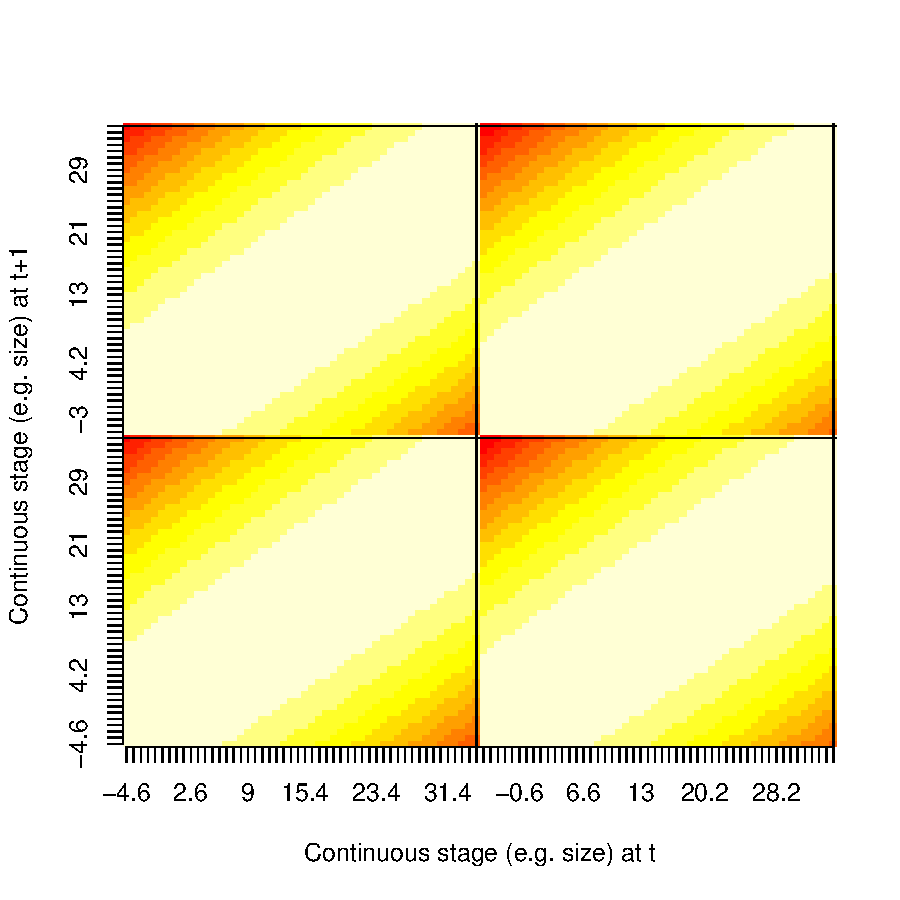
\includegraphics{IPMpack_Vignette-figCompound}
\end{center}
\caption{Compound P matrix IPM shown on a log scale: whiter colours indicate
  more likely transitions; and the four different panels indicate each
  of the four environments.}
\label{fig:five}
\end{figure}
Essentially, the compound P matrix is a large matrix with stacked IPMs
corresponding to each environment, modified to reflect movement
between environmental states defined by {\ env1}. Passage time can be
calculated using a similar function, but now including the environmental
matrix as an argument (equivalent life expectancy functions are in development): 
\begin{Schunk}
\begin{Sinput}
> pTimes <- stochPassageTime(Pmatrix@meshpoints[15], Pmatrix, env1)
\end{Sinput}
\end{Schunk}
The resulting vectors contain the life expectancy and time to reach each size for individuals starting in each different environmental class, concatenated together (i.e. there are {\tt nBigMatrix} values in the LE matrix ranging over the first environment, then {\tt nBigMatrix} values ranging over the second environment, etc). The user can plot these against meshpoints 
(Figure~\ref{fig:five} p.~\pageref{fig:five}), 
each colour indicates a different starting environment. Similar syntax can be used for passage time (although note that here the function name has changed): 
\begin{figure}
\begin{center}
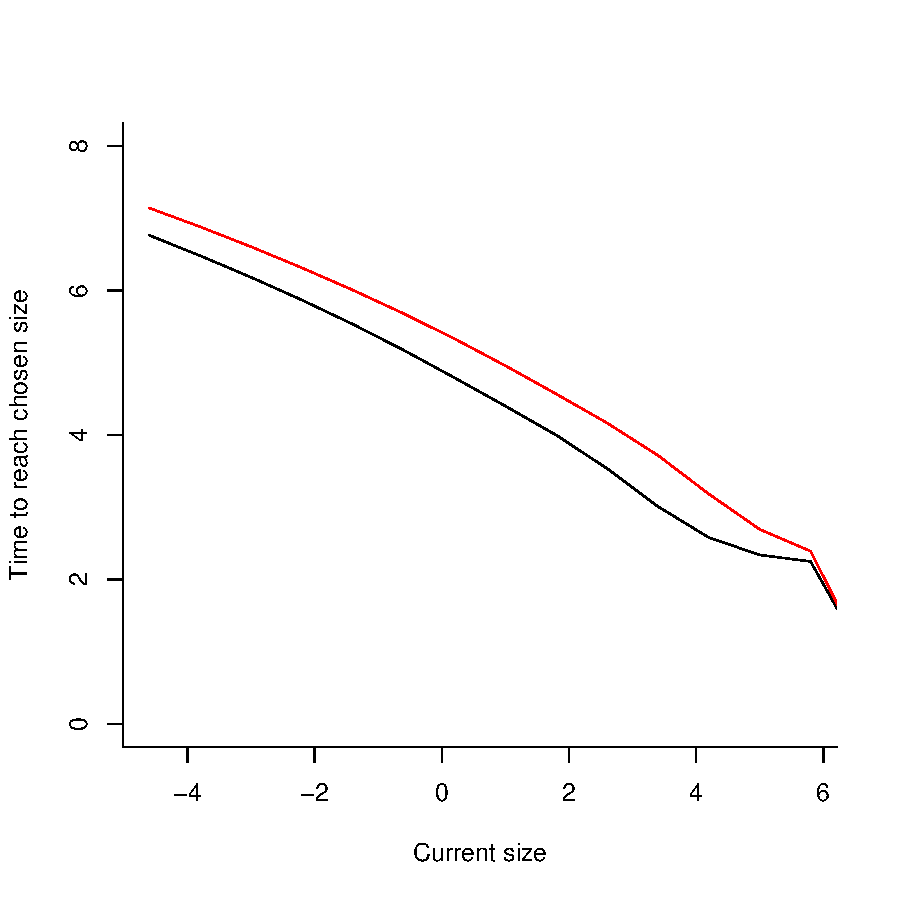
\includegraphics{IPMpack_Vignette-fig5}
\end{center}
\caption{Passage time for a compound IPM;   different colours reflect predictions for individuals starting in different environments}
\label{fig:five}
\end{figure}

Adding a fertility object to this analysis, the user can also define a full life
cycle IPM model for across environments. With such information, obtaining the stochastic population rate of increase $\lambda_s$ in this environment is relatively straight-forward. IPMpack does this by sampling a very large number of environments and corresponding IPMs, and multiplying them together (Childs et al. $2004$). At the moment, this is only defined for the case where environments (defined by the discrete covariates) are distributed independently (i.e. the next state does not depend on the previous state). To do this, the user must first define a list of IPMs (each the sum of a matrix of survival-growth transitions, and a matrix of fecundity transitions corresponding to a particular environment):
\begin{Schunk}
\begin{Sinput}
> IPMlist <- makeListIPMs(dataf = dff, nBigMatrix = 25, minSize = -5, 
+                         maxSize = 35, explSurv = surv~size+covariate, 
+                         explGrow = sizeNext~size+size2+covariate, 
+                         explFec = fec~size, Transform="log",correction = "constant")
\end{Sinput}
\begin{Soutput}
surv ~ size + covariate
\end{Soutput}
\end{Schunk}
Note that in this example IPMpack uses an arbitrary selection of
formulas for the various linear and logistic
regressions ({\tt explGrow}, {\tt explSurv}, etc). In reality,
model selection will need to be used to establish this. Importantly, each
environment type requires sufficient data (years of data) to quantify population
behaviours in that environment as if it were an IPM in a single environment.  
Next, the user can estimate $\lambda_s$ using:
\begin{Schunk}
\begin{Sinput}
> stochGrowthRateSampleList(listIPMmatrix = IPMlist, 
+                           nRunIn = 30, tMax = 50)
\end{Sinput}
\begin{Soutput}
[1] 1.262987
\end{Soutput}
\end{Schunk}
where {\tt nRunIn} defines the number of time steps to discard from the start of the time series in order to remove transient dynamics, and {\tt tMax} is the total
number of time steps to run, and should be large enough that increasing it does not substantially change the result (numbers presented here for efficiency are almost certaintly not large enough). Note that {\tt stoch.growth.rate} in the package {\tt popbio} will operate in essentially the same way, and provides more information, more efficiently.  

%Simply taking the eigenvalue of the sum to the compound $P$ and $F$ matrices will
%provide a sligthly different result given Jensen's inequality. %%check
                                %%this... read Tulja + Carol stoch
                                %%elastivity paper. 

\section{More generally varying environments}

An alternative way of inhabiting stochastic environments is to experience continuously changing covariates (rather than moving between discrete states, as the above describes). In this case, rather than building a single megamatrix, desired variables are obtained by multiplying up a suite of matrices and relying on the weak
ergodic theorem for convergence (e.g., Tuljapurkar 1990; as described for obtaining $\lambda_s$, above). IPMpack contains code to do this. The user must first define a new data frame containing several time-varying covariates, and then, build the associated survival, growth and fertility objects (note that the default in IPMpack is to assume that if you have a covariate called "coviariate", your aim is to build a compound matrix, so ideally other covariates should have other names): 
\begin{Schunk}
\begin{Sinput}
> dff <- generateDataStoch()
> sv1 <- makeSurvObj(dataf = dff, 
+                           Formula = surv~size+covariate1+covariate3)
> gr1 <- makeGrowthObj(dataf = dff, 
+                              Formula = sizeNext~size+covariate1+covariate2)
> fv1 <- makeFecObj(dataf = dff, fecConstants = data.frame(1.8), 
+                   Formula = fec~size, Transform = "log")
\end{Sinput}
\end{Schunk}
As before, the user can explore the data: 
\begin{Schunk}
\begin{Sinput}
> head(dff)
\end{Sinput}
\begin{Soutput}
      size   sizeNext surv covariate1  covariate2 covariate3        fec
1 6.954512  4.6997744    1 -0.8285339  0.08481277  0.1635935 10.5150795
2 6.460448  6.9801350    1  0.1801215 -2.60995838 -1.0368096  0.0000000
3 3.406381  6.2496965    1  0.7769606 -1.34793803  0.6472874 22.1744621
4 3.851654         NA    0  0.8109758  1.52100342  1.6534940 13.0232382
5 6.548206         NA    0  1.1935911  1.75016426  0.3656397  0.1001767
6 5.240481 -0.8170451    1 -2.2038146 -0.32884894  0.4172472  9.1633087
       stage  stageNext number
1 continuous continuous      1
2 continuous continuous      1
3 continuous continuous      1
4 continuous continuous      1
5 continuous continuous      1
6 continuous continuous      1
\end{Soutput}
\end{Schunk}
and glance at the objects, e.g., 
\begin{Schunk}
\begin{Sinput}
> gr1
\end{Sinput}
\begin{Soutput}
An object of class "growthObj"
Slot "fit":

Call:
lm(formula = Formula, data = dataf)

Coefficients:
(Intercept)         size   covariate1   covariate2  
   0.964549     0.903368     2.998632     0.005781  


Slot "sd":
[1] 0.2203201
\end{Soutput}
\end{Schunk}
To explore demographic projections for this model, the user must decide on
a time scale and time length, and define it by a vector called
`tVals'.  This time series can be used to reflect patterns in environmental data
that repeat.  In this example we set {\tt tVals} to reflect monthly intervals
over $4$ years, with years as the time scale and build covariates that vary
seasonally, i.e., they fluctuates randomly around a sine wave which peaks once a
year.  From this simulation, the user can generate a matrix containing time as
rows and different covariates in columns.
\begin{Schunk}
\begin{Sinput}
> tVals <- seq(1, 4, by = 1/12)
> covTest <- c(1 + 0.5*sin(2*pi*tVals))
> covMatTest <- data.frame(covariate1 = rnorm(length(covTest), covTest, 0.5) - 1, 
+                          covariate2 = rnorm(length(covTest), covTest, 0.5) - 1, 
+                          covariate3 = rnorm(length(covTest), covTest, 0.5) - 1)
\end{Sinput}
\end{Schunk}
Note that  if there is no apparent temporal pattern to the data, one could
simply generate random normal distributions of the covariates using their observed mean and variance. Other types of temporal patterns (multiannual, etc) are also possible. With this setup, the user can then estimate the stochastic growth rate over these years, using the geometric mean of the population growth rate (Tuljapurkar $1990$; Childs et al. $2004$), for these particular covariates using:
\begin{Schunk}
\begin{Sinput}
> r <- stochGrowthRateManyCov(covariate = covMatTest, nRunIn = 12*1, 
+                             tMax = length(tVals), growthObj = gr1, 
+                             survObj = sv1, fecObj = fv1, nBigMatrix = 20, 
+                             minSize = 2*min(dff$size, na.rm = TRUE), 
+                             maxSize = 1.5*max(dff$size, na.rm = TRUE), 
+                             nMicrosites = 50, correction = "constant")
> print(r)
\end{Sinput}
\begin{Soutput}
[1] -0.01534196
\end{Soutput}
\end{Schunk}
Setting nRunIn = $12*1$ in this example is equivalent to discarding the first 
year of the simulation (likely to contain transients) since the chosen time step
is months.Note that in this formula, it was assumed that density-dependence acts on
seedling establishment, and that $50$ microsites are available for seedling establishment in every time step. Setting nMicrosites = $0$ allows for calculations without density-dependence, and nMicrosites can also be a vector, if the number of microsites fluctuates through time. It may also be interesting to have a glance at what has been happening to the population structure over this time-course, and the function {\tt trackPopStructManyCov} allows this. IPMpack also contains a dedicated function to depict the results from this, {\tt plotResultsStochStruct}.


\section{Parameter uncertainty in a constant environment}

To illustrate parameter uncertainty in a constant environment, we
generate data again, and from these data build a list of survival and growth
objects reflecting the parameter posteriors of fitted linear and logistic
regression models (taking the simplest case of structure only via a continuous
covariate). Note that it is also possible (and simpler) to directly use the variance-covariance of parameters estimates from a maximum-likelihood fit (via {\tt glm} or {\tt lm}) to build a list of growth, survival or fertility objects reflecting parameter uncertainty (see the help file for {\tt getListRegObjects}) but here we illustrate the Bayesian case.
\begin{Schunk}
\begin{Sinput}
> dff <- generateData()
> grlist <- makePostGrowthObjs(dff, 
+                              explanatoryVariables = "size", 
+                              burnin = 100, nitt = 400)
> svlist <- makePostSurvivalObjs(dff, 
+                                explanatoryVariables = "size", 
+                                burnin = 100, nitt = 400)
\end{Sinput}
\end{Schunk}
This function currently only uses default non-informative priors features. There is a default thinning in MCMCglmm, the engine used to derive the posteriors, that reduces simulations by 10. So the number of samples from the posterior used in this simple example
{\tt nitt} is rather small (resulting in only [nitt - burnin] / 10 = 30), and
larger numbers are advisable (the default in MCMCglmm is 50,000). With output from this, the user can make a list containing multiple P matrices:
\begin{Schunk}
\begin{Sinput}
> PmatrixList <- makeListPmatrix(grlist, svlist, nBigMatrix = 20, 
+                                minSize = -5, 
+                                maxSize = 35, 
+                                correction = "constant")
\end{Sinput}
\end{Schunk}
If one of the lists is longer than the other, this function samples the shorter object at random to reach the size of the longer object. Note that in this example the matrix size is rather small just to save time, and larger number of bins are advisable. The function will also construct compound matrices, if an environmental matrix is provided. With this, the user can now obtain  posteriors for constant environment models. 
\begin{Schunk}
\begin{Sinput}
> res <- getIPMoutput(PmatrixList, targetSize = 5, FmatrixList = NULL)
> names(res)
\end{Sinput}
\begin{Soutput}
[1] "LE"          "pTime"       "lambda"      "stableStage"
\end{Soutput}
\end{Schunk}
The vector called $\lambda$ and matrix called stableSize, etc, will consist of
NAs, unless a list of Fmatrices is also provided, which would allow a complete
population projection matrix to be built. IPMpack contains a similar function to obtain a list of F matrices, and if such a list is included as the third argument into the function {\tt getIPMOutput} (for which the default is `NULL'), the function will also return distributions of $\lambda$, the stable stage distribution, etc:
\begin{Schunk}
\begin{Sinput}
> fv <- makePostFecObjs(dff, explanatoryVariables = "size+size2", fecConstants=data.frame(0.01), 
+                       burnin = 100, nitt = 400, Transform = "log")
\end{Sinput}
\begin{Soutput}
[1] 30
\end{Soutput}
\begin{Sinput}
> FmatrixList <- makeListFmatrix(fv, nBigMatrix = 20, minSize = -5, 
+                                maxSize = 35, cov = FALSE,
+                                correction = "constant")
> res <- getIPMoutput(PmatrixList, targetSize = 5, FmatrixList)
\end{Sinput}
\end{Schunk}

Again, larger numbers of iterations, binsizes, etc, are recommended. These results
can be visually inspected too (Figure~\ref{fig:seven} p.~\pageref{fig:seven}):
\begin{figure}
\begin{center}
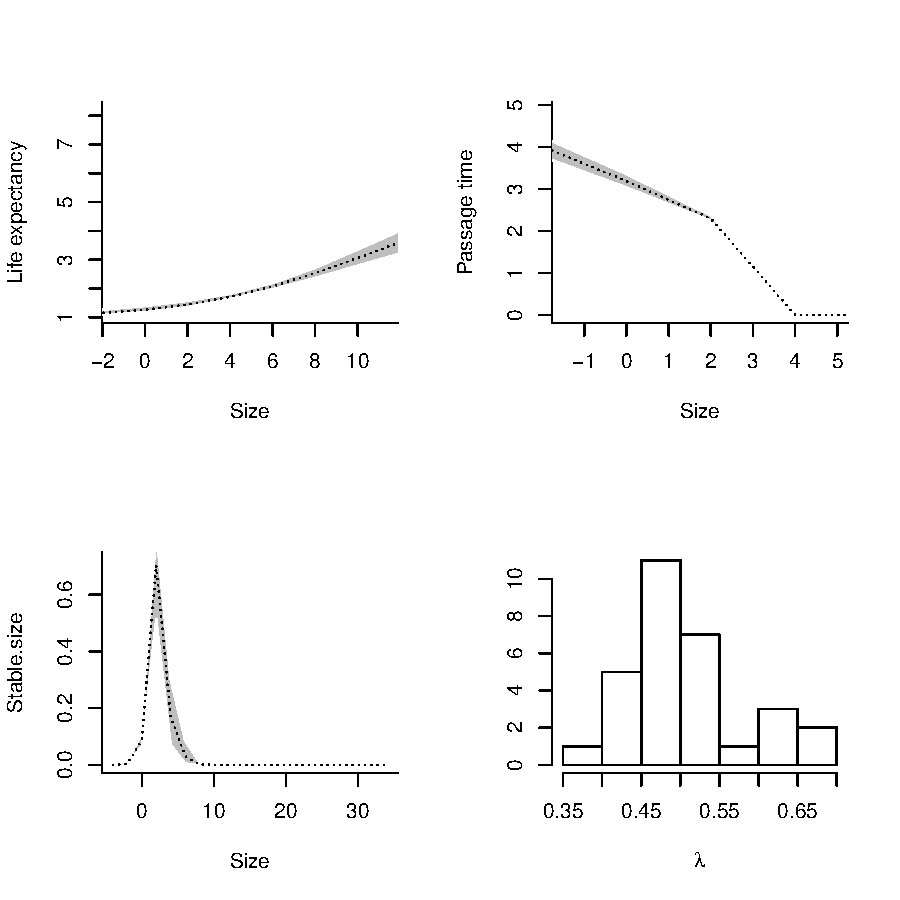
\includegraphics{IPMpack_Vignette-fig7}

\end{center}
\caption{Uncertainty in IPM output}
\label{fig:seven}
\end{figure}

This is a rather slow way of proceeding - a large number of IPMs are being
stored in R's memory. A slightly more rapid approach is to use the function {\tt
getIPMOutputDirect} that builds an IPM from a sample from the posterior,
calculates relevant parameters, then over-writes this with a rebuilt IPM,
iterating though the list.


\section{Building your own objects and methods}
What if growth is best reflected by a saturating function, rather than by the
linear regression models provided?  In this case the user may want to define a
new class of growth object.  An example of this follows:
\begin{Schunk}
\begin{Sinput}
> setClass("growthObjSaturate", representation(paras = "numeric", sd = "numeric"))
\end{Sinput}
\end{Schunk}
Then define the functional form of the mean prediction, with relevant parameters: 
\begin{Schunk}
\begin{Sinput}
> fSaturate <- function(size, pars) { 
+     u <- exp(pmin(pars[1] + pars[2] * size, 50))
+     u <- pars[3] * 1/(1+u)
+     return(u)
+ }
\end{Sinput}
\end{Schunk}
where the third parameter indicates the asymptotic size. The user can then
estimate the parameters by fitting this function to the data using a wrapper
function and the R function {\tt optim}.
\begin{Schunk}
\begin{Sinput}
> wrapSaturate <- function(par, dataf) { 
+     pred <- fSaturate(dataf$size, par[1:3])
+     ss <- sum((pred - dataf$sizeNext)^2, na.rm = TRUE)
+     return(ss)
+     }
> tmp <- optim(c(1, 1, 1), wrapSaturate, dataf = dff, method = "Nelder-Mead")
> tmp    
\end{Sinput}
\begin{Soutput}
$par
[1]  2.101137 -0.377573  9.447406

$value
[1] 601.5573

$counts
function gradient 
     294       NA 

$convergence
[1] 0

$message
NULL
\end{Soutput}
\end{Schunk}

For simplicity, one can assume normally distributed errors: 

\begin{Schunk}
\begin{Sinput}
> resids <- fSaturate(dff$size, tmp$par) - dff$sizeNext
> sdSaturate <- sd(resids, na.rm = TRUE)
\end{Sinput}
\end{Schunk}

With these parameters, the user can then define the new growth object:

\begin{Schunk}
\begin{Sinput}
> gr1 <- new("growthObjSaturate")
> gr1@paras <- tmp$par
> gr1@sd <- sdSaturate
\end{Sinput}
\end{Schunk}

Finally, the user must define a method appropriate for this type of object. 

\begin{Schunk}
\begin{Sinput}
> setMethod("growth", c("numeric", "numeric", "numeric", "growthObjSaturate"), 
+           function(size, sizeNext, cov, growthObj){
+               mux <- fSaturate(size, growthObj@paras)
+               sigmax <- growthObj@sd
+               u <- dnorm(sizeNext, mux, sigmax, log = F)  
+               return(u);
+           })
\end{Sinput}
\begin{Soutput}
[1] "growth"
\end{Soutput}
\end{Schunk}
By putting {\tt growthObjSaturate} in the signature, R will use this particular method for all objects with this signature. Now, the user can go ahead and use all the other code as previously, without a need for further definitions. 

If the user wishes to fit a growth model with, for example, gamma errors, a similar approach can be used, but with `dgamma' instead of dnorm in the last line of growth method, and appropriate slots defined in the object, etc. 

\section*{Selected References}



\begin{itemize}
\item Caswell. 2001. Matrix population models: analysis, construction and interpretation. 2nd ed. Sinauer. Massachussetts, USA.

\item Childs, Rees, Rose, Grubb \& Ellner. 2004. Evolution of size-dependent flowering in a variable environment: Construction and analysis of a stochastic integral projection model. Proc. Roy. Soc. Lond. Ser. B. 271: 471-475.

\item Cochran \& Ellner. 1995. Simple methods for calculating age-based life history parameters for stage-structured populations. Ecological Monographs 62: 345-364.

\item Ellner \& Rees. 2006. Integral projection models for species with complex life-histories. American Naturalist 167: 410-428.

\item Metcalf, Horvitz, Tuljapurkar \& Clark. 2009. A time to grow and a time to die: a  new way to analyze the dynamics of size, light, age and death of tropical trees. Ecology 90: 2766-2778.

\item Rees \& Rose. 2002. Evolution of flowering strategies in Oenothera glazioviana: an integral projection model approach. Proc. Roy. Soc. Lond. Ser. B. 269: 1509-1515.

\item Ramula, Rees \& Buckley. 2009. Integral projection models perform better for small demographic data sets than matrix population models: a case study of two perennial herbs. Journal of Applied Ecology 46: 1048-1053.

\item Salguero-Gomez \& Plotkin. 2010. Matrix dimensionality bias demographic inferences: implications for comparative plant demography. The American Naturalist 176: 710-722

\item Tuljapurkar. 1990. Population Dynamics in Variable Environments. Springer. New York, USA.

\item Zuidema, Jongejans, Chien, During \& Schieving. 2010. Integral Projection Models for trees: a new parameterization and a validation of model output. Journal of Ecology 98: 345-355.


\end{itemize}

%\section{Extensions}

%\begin{itemize}
%\item  sensitivity / elasticity a la Carol Tulja
%\item stable size dist in stoch env
%\item survivorship in a stochastic environment
%\item density dependence generic functions
%\item age structure
%\item jim style multi-year census interval growth bayes
%\item loop analysis (see Zuidema in Ecology showing fast growing
%  trees contribute more)
%\end{itemize}


\end{document}

